\documentclass[12pt,a4paper]{extreport}
\usepackage[l2tabu,orthodox]{nag}

\usepackage[left=15mm,right=15mm, top=20mm,bottom=20mm,bindingoffset=0cm]{geometry}

\usepackage{indentfirst}
\usepackage[labelsep=period]{caption}
\usepackage{amssymb,amsmath,amsthm}
\usepackage{fontspec}
\usepackage{float}
\usepackage{array}
\usepackage{listings}


\setmainfont[Ligatures=TeX]{STIX}
\newfontfamily{\cyrillicfont}[Ligatures=TeX]{STIX}
\setmonofont{Fira Mono}
\newfontfamily{\cyrillicfonttt}{Fira Mono}

\usepackage{polyglossia}
\setdefaultlanguage{russian}
\setotherlanguage{english}

\usepackage{subcaption}
\usepackage{graphicx}
\graphicspath{img/}
\DeclareGraphicsExtensions{.pdf,.png,.jpg}

\usepackage{color}
\definecolor{darkblue}{rgb}{0,0,.75}
\definecolor{darkred}{rgb}{.7,0,0}
\definecolor{darkgreen}{rgb}{0,.7,0}

\usepackage[normalem]{ulem}
\setlength{\marginparwidth}{2cm}
\usepackage[textwidth=4cm,textsize=tiny]{todonotes}
\newcommand{\fix}[2]{{\textcolor{red}{\uwave{#1}}\todo[fancyline]{#2}}}
\newcommand{\hl}[1]{{\textcolor{red}{#1}}}
\newcommand{\cmd}[1]{{\ttfamily{\textbackslash #1}}}

\newcommand{\vrb}[1]{\PVerb{#1}}
\newcommand{\vrbb}[1]{\texttt{\textbackslash}\PVerb{#1}}

\usepackage[
    draft = false,
    unicode = true,
    colorlinks = true,
    allcolors = blue,
    hyperfootnotes = true
]{hyperref}

\usepackage{tikz}
\usetikzlibrary{graphs, quotes}
\usepackage{relsize}
\usepackage{ytableau}

%\usepackage{titlesec}
%\titleformat{\subsection}{\normalfont\large\bfseries}{\thesubsection.}{\smallskip}{}
\renewcommand \thesection{\Roman{section}}
\renewcommand \thesubsection{\arabic{subsection}}

\theoremstyle{plain}
\newtheorem{theorem}{Теорема}
\newtheorem{lemma}{Лемма}
\newtheorem{proposition}{Утверждение}
\newtheorem{corollary}{Следствие}
\theoremstyle{definition}
\newtheorem{definition}{Определение}
\newtheorem{notation}{Обозначение}
\newtheorem{example}{Пример}
\newcommand\abs[1]{\left\lvert #1 \right\rvert}
\newcommand\ceil[1]{\left\lceil{#1}\right\rceil}
\newcommand\floor[1]{\left\lfloor{#1}\right\rfloor}
\newcommand{\divby}{\;\raisebox{-0.4ex}{\vdots}\;} 

\title{<<Самостоятельная работа по подготовке к ВПР 5-го класса>>}
\begin{document}
\maketitle
\pagebreak


Давайте продифференцируем данную легчайшую функцию.

\begin{equation*}
f(x) = \sin(15 \cdot {x}^{3}) + ({\cos(20 \cdot x + 1))}^{3}
\end{equation*}


Приступаем к дифференцированию.

\begin{equation*}
f'(x) = \cos(15 \cdot {x}^{3}) \cdot 0 \cdot {x}^{3} + 15 \cdot 3 \cdot {x}^{3 - 1} + 3 \cdot \sin(20 \cdot x + 1) \cdot 0 \cdot x + 20 \cdot 1 + 0 \cdot -1 \cdot ({\cos(20 \cdot x + 1))}^{2}
\end{equation*}
Давайте немного упростим данное выражение.

\begin{equation*}
f'_{\text{упрощённая}} = \cos(15 \cdot {x}^{3}) \cdot 15 \cdot 3 \cdot {x}^{2} + 3 \cdot \sin(20 \cdot x + 1) \cdot 20 \cdot -1 \cdot ({\cos(20 \cdot x + 1))}^{2}
\end{equation*}


Несложно заметить, что графики выглядят так:

\begin{minipage}{0.45\textwidth}
\centering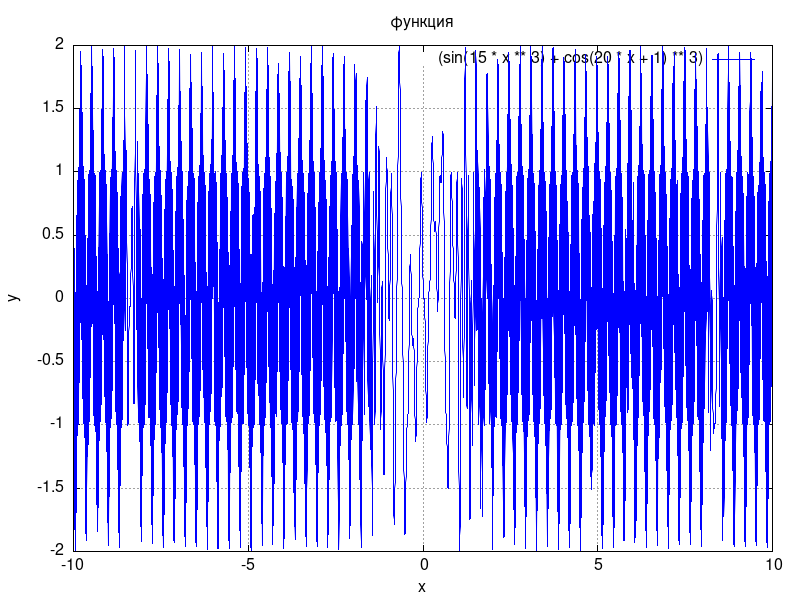
\includegraphics[width=\linewidth]{orig_plot.png}\end{minipage}
\hfill
\begin{minipage}{0.45\textwidth}
\centering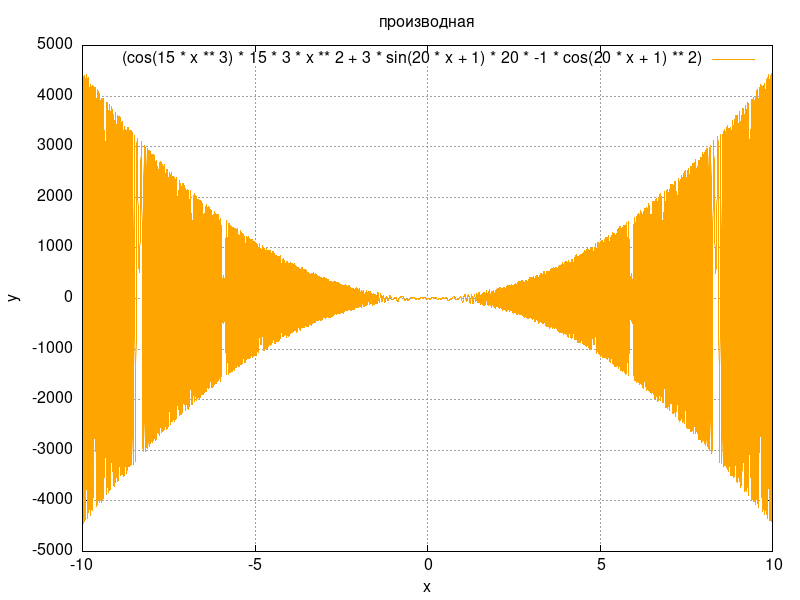
\includegraphics[width=\linewidth]{optimized_plot.png}\end{minipage}
\end{document}
